\pgfsetplotmarksize{0pt}
 \centering
 \caption{\label{CBCvsMSTAV-d05}CBCvsMSTAV-d05},
 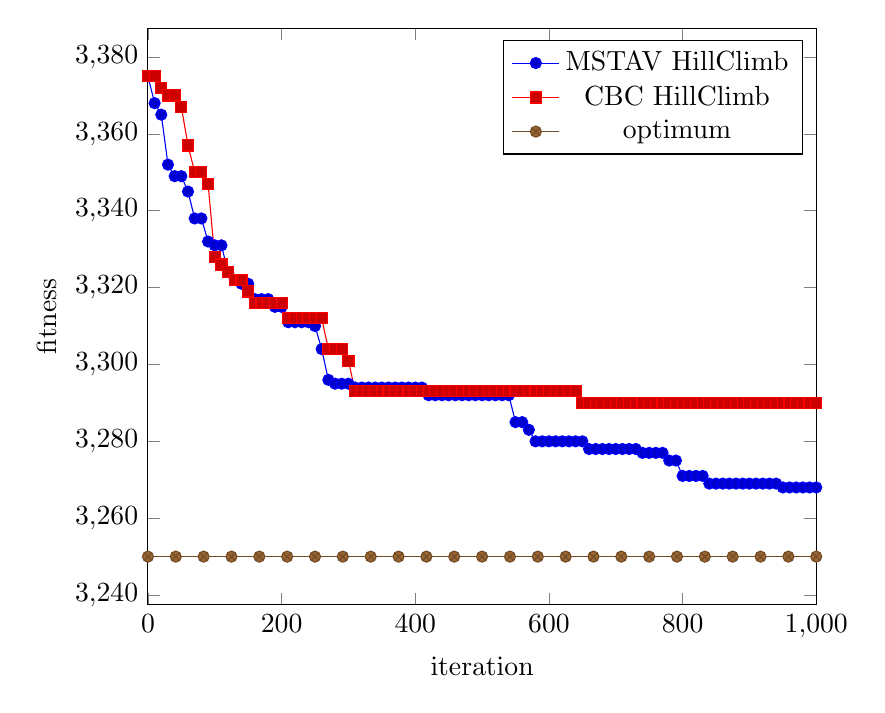
\begin{tikzpicture}
 \begin{axis}[
   width=0.7\textwidth,
   scale only axis,
   xlabel=iteration,
   ylabel=fitness,
   xmin=0,xmax=1000,
   domain=0:1000]
   \addplot coordinates {
     (0,3375)
     (10,3368)
     (20,3365)
     (30,3352)
     (40,3349)
     (50,3349)
     (60,3345)
     (70,3338)
     (80,3338)
     (90,3332)
     (100,3331)
     (110,3331)
     (120,3324)
     (130,3322)
     (140,3321)
     (150,3321)
     (160,3317)
     (170,3317)
     (180,3317)
     (190,3315)
     (200,3315)
     (210,3311)
     (220,3311)
     (230,3311)
     (240,3311)
     (250,3310)
     (260,3304)
     (270,3296)
     (280,3295)
     (290,3295)
     (300,3295)
     (310,3294)
     (320,3294)
     (330,3294)
     (340,3294)
     (350,3294)
     (360,3294)
     (370,3294)
     (380,3294)
     (390,3294)
     (400,3294)
     (410,3294)
     (420,3292)
     (430,3292)
     (440,3292)
     (450,3292)
     (460,3292)
     (470,3292)
     (480,3292)
     (490,3292)
     (500,3292)
     (510,3292)
     (520,3292)
     (530,3292)
     (540,3292)
     (550,3285)
     (560,3285)
     (570,3283)
     (580,3280)
     (590,3280)
     (600,3280)
     (610,3280)
     (620,3280)
     (630,3280)
     (640,3280)
     (650,3280)
     (660,3278)
     (670,3278)
     (680,3278)
     (690,3278)
     (700,3278)
     (710,3278)
     (720,3278)
     (730,3278)
     (740,3277)
     (750,3277)
     (760,3277)
     (770,3277)
     (780,3275)
     (790,3275)
     (800,3271)
     (810,3271)
     (820,3271)
     (830,3271)
     (840,3269)
     (850,3269)
     (860,3269)
     (870,3269)
     (880,3269)
     (890,3269)
     (900,3269)
     (910,3269)
     (920,3269)
     (930,3269)
     (940,3269)
     (950,3268)
     (960,3268)
     (970,3268)
     (980,3268)
     (990,3268)
     (1000,3268)
   };
   \addlegendentry{MSTAV HillClimb}
   \addplot coordinates {
     (0,3375)
     (10,3375)
     (20,3372)
     (30,3370)
     (40,3370)
     (50,3367)
     (60,3357)
     (70,3350)
     (80,3350)
     (90,3347)
     (100,3328)
     (110,3326)
     (120,3324)
     (130,3322)
     (140,3322)
     (150,3319)
     (160,3316)
     (170,3316)
     (180,3316)
     (190,3316)
     (200,3316)
     (210,3312)
     (220,3312)
     (230,3312)
     (240,3312)
     (250,3312)
     (260,3312)
     (270,3304)
     (280,3304)
     (290,3304)
     (300,3301)
     (310,3293)
     (320,3293)
     (330,3293)
     (340,3293)
     (350,3293)
     (360,3293)
     (370,3293)
     (380,3293)
     (390,3293)
     (400,3293)
     (410,3293)
     (420,3293)
     (430,3293)
     (440,3293)
     (450,3293)
     (460,3293)
     (470,3293)
     (480,3293)
     (490,3293)
     (500,3293)
     (510,3293)
     (520,3293)
     (530,3293)
     (540,3293)
     (550,3293)
     (560,3293)
     (570,3293)
     (580,3293)
     (590,3293)
     (600,3293)
     (610,3293)
     (620,3293)
     (630,3293)
     (640,3293)
     (650,3290)
     (660,3290)
     (670,3290)
     (680,3290)
     (690,3290)
     (700,3290)
     (710,3290)
     (720,3290)
     (730,3290)
     (740,3290)
     (750,3290)
     (760,3290)
     (770,3290)
     (780,3290)
     (790,3290)
     (800,3290)
     (810,3290)
     (820,3290)
     (830,3290)
     (840,3290)
     (850,3290)
     (860,3290)
     (870,3290)
     (880,3290)
     (890,3290)
     (900,3290)
     (910,3290)
     (920,3290)
     (930,3290)
     (940,3290)
     (950,3290)
     (960,3290)
     (970,3290)
     (980,3290)
     (990,3290)
     (1000,3290)
   };
   \addlegendentry{CBC HillClimb}
   \addplot {3250.000000};
   \addlegendentry{optimum}
 \end{axis}
 \end{tikzpicture}
